\chapter{Design di Dettaglio}

In questo capitolo vengono analizzate le scelte operate a livello di design nel dettaglio. In particolare viene analizzata la struttura data a ciascuno dei servizi ed i principali pattern di progettazione adottati.

\section{Suddivisione in moduli}

Il nostro progetto è stato suddiviso in moduli in quanto permette un'organizzazione \textit{by-need} dei singoli moduli. Questo permette ad ogni modulo di includere come dipendenza solo i moduli di cui necessita, ottimizzando l'incapsulamento.

I moduli definiti sono:

\begin{itemize}
%
    \item \textit{Commons}: contiene tutte le parti di codice riutilizzate all'interno dei diversi moduli.
%
    \item \textit{Data Access}: contiene tutte le parti di codice riutilizzate per l'accesso (in lettura e scrittura) ad una base di dati relazionale.
%
    \item \textit{Exceptions}: contiene una rappresentazione di tutte le eccezioni di dominio e fornisce costrutti utili per la loro gestione.
%
    \item \textit{Interactors}:  contiene i costrutti comuni per la creazione di casi d'uso.
%
    \item \textit{Service Commons}: contiene i costrutti comuni per la creazione, pubblicazione e scoperta di servizi.
%
\end{itemize}

\section{Parti comuni}

In questa sezione vengono descritte le parti di codice comune che vengono riutilizzate all'interno di altri moduli.

\subsection{Commons}

All'interno del modulo \textit{Commons} sono state fattorizzate principalmente:

\begin{itemize}
%
    \item Alcune funzionalit\`a generiche:
    \begin{itemize}
%
        \item logging;
%
        \item lettura di file.
%
    \end{itemize}
%
    \item Funzionalit\`a per agevolare la trasformazione da oggetti descritti in formato \textit{JSON} a costrutti Scala.
%
    \item Funzionalit\`a per la conversione da costrutti di Vert.x a \texttt{Scheduler} RxScala e classi implicite per arricchire gli \texttt{Observable} RxScala con funzionalit\`a aggiuntive.
%
    \item Funzionalit\`a per convertire una chiamata asincrona ad un metodo fornito da Vert.x in un \texttt{Observable} RxScala, metodi di conversione e utilizzo del pattern  \textbf{Pimp my Library} per arricchire di nuove funzionalit\`a le classi \texttt{AsyncResult}, \texttt{EventBus} e \texttt{Json}.
%
    \item Funzionalit\`a per agevolare l'estrazione di parametri dal contesto di una richiesta HTTP e una classe implicita per estendere il costrutto \texttt{HttpServerResponse} di Vert.x.
%
    \item Altri costrutti pi\`u avanzati sono descritti in dettaglio nelle successive sotto-sezioni.
%
\end{itemize}

\begin{figure}[H]
  \centering
    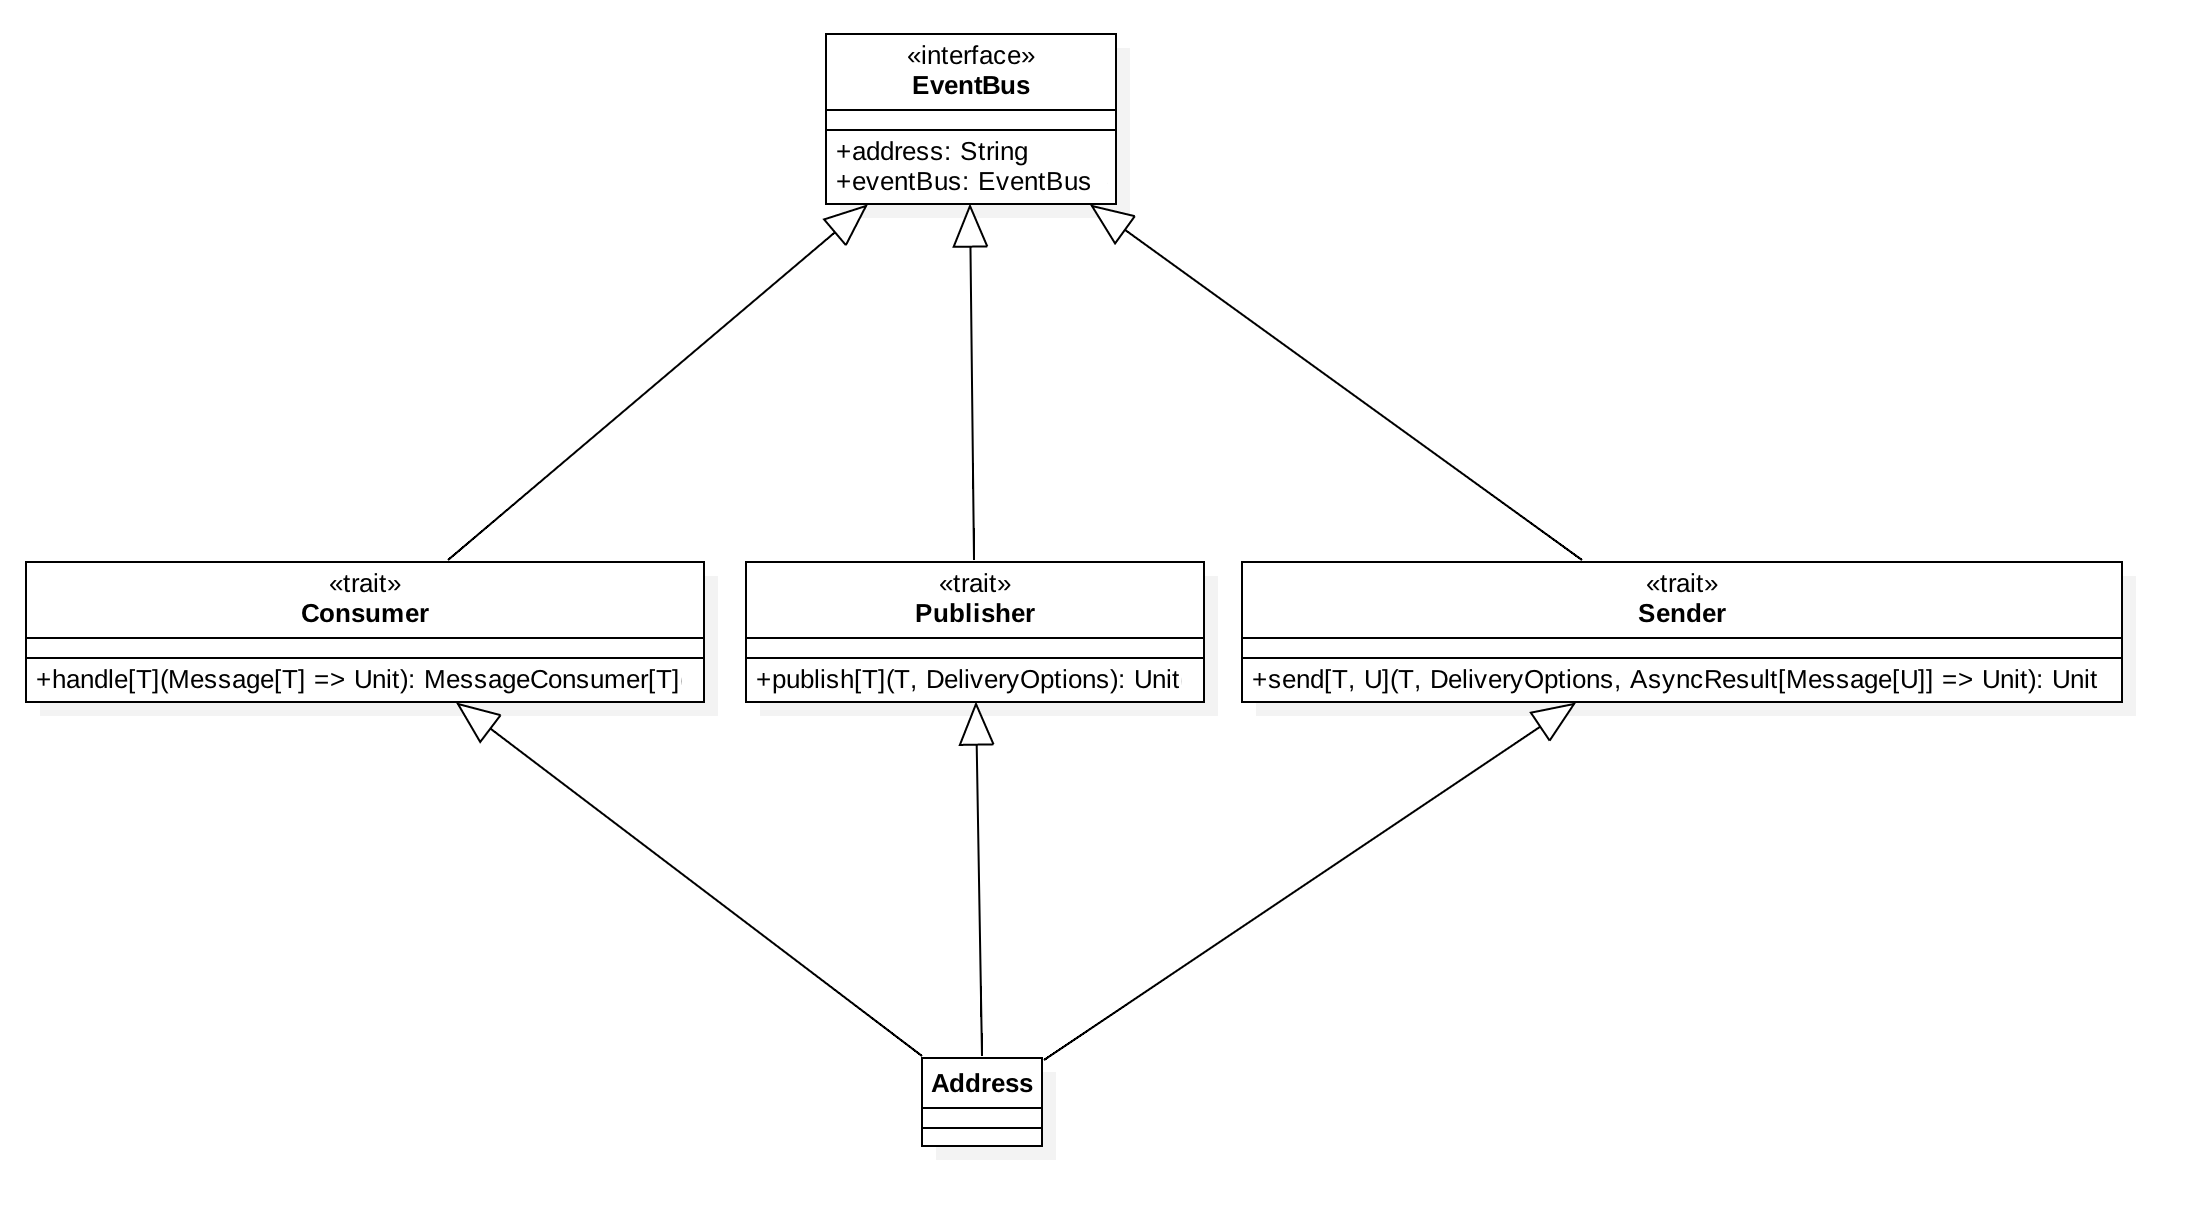
\includegraphics[width=\linewidth, height=\textheight, keepaspectratio]{AddressClassDiagram}
  \caption{Utilizzo del \textit{mix-in} per aggiungere funzionalit\`a alla classe \texttt{Address}.}
\end{figure}

\subsubsection{Validazione}

Per realizzare la validazione dell'input utente è stato utilizzato il pattern \textit{builder}.
%
La scelta di utilizzare questo pattern progettuale \`e legata al fatto che non \`e possibile determinare a priori quante (e quali) regole dovranno essere applicate per effettuare la validazione di un input.

La classe \texttt{ValidatorBuilder} \`e incaricata di gestire la costruzione di un oggetto \texttt{Validator}, per fare ciò \`o espone il metodo \texttt{addRule} che permette di aggiungere al builder un ulteriore regola di validazione.
%
\texttt{ValidatorBuilder} espone due overload del metodo \texttt{addRule}, il primo prende in input una regola da applicare, il secondo prende in input un predicato e un'eccezione da sollevare nel caso l'oggetto passato in input al validatore non sia soddisfatta.

Per la creazione di oggetti di tipo \texttt{Validator} \`e stato utilizzato il pattern \textit{Execute Around} che permette, tramite un espressione lambda, di eseguire un blocco di codice ed incapsulare all'interno del metodo eventuali operazioni di creazione e \textit{clean-up}.

\begin{figure}[H]
  \centering
    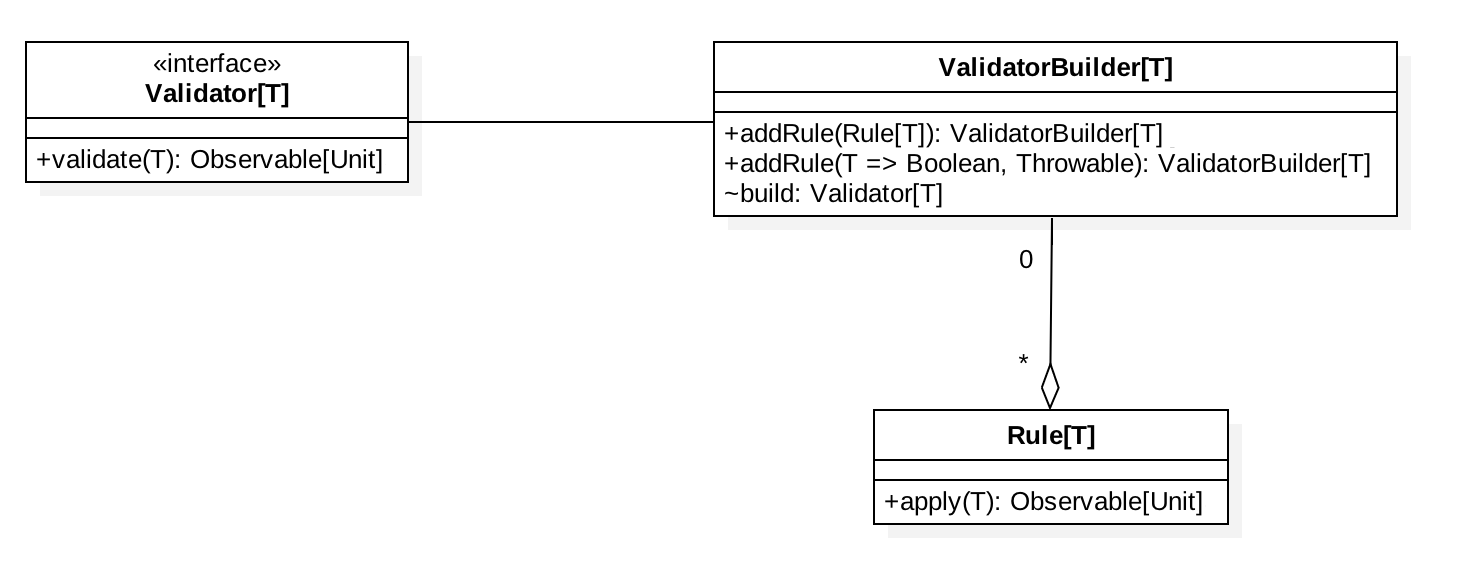
\includegraphics[width=\linewidth, height=\textheight, keepaspectratio]{ValidationClassDiagram}
  \caption{Diagramma delle classi per la classe per la costruzione di un \texttt{Validator}.}
\end{figure}

\subsubsection{Configurazione}

Per gestire la configurazione di oggetti complessi è stata utilizzata la classe \texttt{Configurator}, la quale permette di applicare in cascata un insieme di funzioni ad un'istanza passata in input.

\subsection{Data Access}

All'interno del modulo \textit{Data Access} sono state inserite tutte le parti di codice che sono state riutilizzate all'interno di altri moduli per semplificare l'interazione con la base di dati sottostante, inoltre espone alcune conversioni per agevolare la traduzione di tipi di dato Scala in tipi di dato interpretabili MySQL (nello specifico \texttt{Boolean} e \texttt{java.util.Date}).
%
Utilizzo del pattern \textbf{Pimp my Library} per arricchire la classe \texttt{ResultSet} aggiungendovi un metodo che permette di ottenere una rappresentazione JSON di ogni record restituito dall'interrogazione.

\subsection{Exceptions}

All'interno del modulo \textit{Exceptions} sono contenute tutte le possibili eccezioni che l'applicazione potrebbe sollevare. Fornisce metodi utili per la conversione delle eccezioni in oggetti JSON (e viceversa), oltre ad un metodo per determinare il tipo di errore HTTP a partire dall'eccezione sollevata.

\subsection{Interactors}

All'interno del modulo \textit{Interactors} sono contenuti i costrutti comuni per la creazione di casi d'uso.

La classe \texttt{UseCase}, classe padre di tutti i casi d'uso, sfrutta il pattern progettuale \textit{Template method} per raccogliere a fattor comune le modalit\`a di interazione e lasciare alle sottoclassi la definizione del comportamento.

\begin{figure}[H]
  \centering
    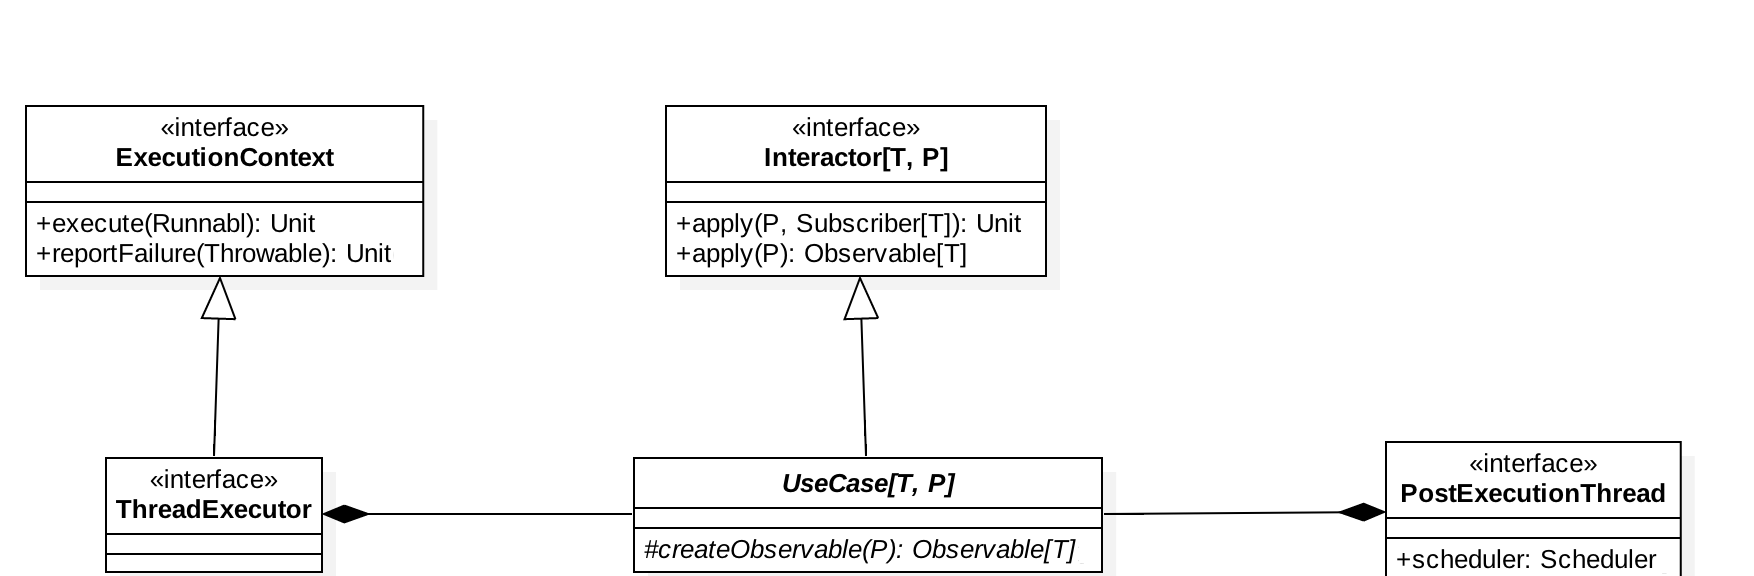
\includegraphics[width=\linewidth, height=\textheight, keepaspectratio]{UseCaseClassDiagram}
  \caption{Diagramma delle classi per la classe \texttt{UseCase}.}
\end{figure}

\subsection{Service Commons}

All'interno del modulo \textit{Service Commons} sono contenuti i costrutti comuni per la definizione, pubblicazione e scoperta di un servizio.

\`E utilizzato il pattern \textit{Template method} nella classe \texttt{ServiceVerticle} al fine di raccogliere a fattor comune le modalit\`a di inizializzazione del componente e demandare alle sottoclassi la definizione delle proprie rotte.

\section{Suddivisione dei servizi}

Nel nostro progetto abbiamo rispettato il pattern architetturale di suddivisione del progetto a \textit{microservizi} (come discusso nel capitolo 3), in quanto fornisce notevoli vantaggi rispetto al classico approccio dell'applicativo server monolitico.
%
Di seguito verranno elencati tutti i servizi del progetto, per poi andare ad analizzarli nel dettaglio nelle sezioni successive:

\begin{itemize}
%
    \item \textit{Authentication Service}: gestisce l'accesso, la registrazione, il logout e l'autenticazione delle richieste effettuate da un utente.
%
    \item \textit{Room Service}: gestisce la creazione e l'eliminazione di una stanza, la partecipazione di un utente in una stanza e la persistenza dei messaggi scambiati in ciascuna stanza.
%
    \item \textit{User Service}: gestisce la creazione, eliminazione e modifica dei profili utente.
%
    \item \textit{Web App Service}: funge da intermediario fra i client e i servizi di cui sopra. 
%
\end{itemize}

\subsection{Scelte rilevanti}

Durante la fase di analisi del problema abbiamo ritenuto opportuno che ogni microservizio avesse una sua specifica visione del dominio, in modo tale che ognuno lo vedesse al proprio livello di dettaglio d'interesse. Questa scelta ha portato ad una duplicazione consapevole di alcune entità del dominio.
\\
Per validare le richieste ricevute i servizi usufruiscono di casi d'uso ausiliari. Tale scelta consente di non ``sporcare'' l'implementazione del caso d'uso principale e favorire il riuso dello stesso validatore per richieste effettuate a casi d'uso diversi.
\\
Laddove si è ritenuto vantaggioso è stato applicato il pattern \textbf{Factory Method} utilizzando i \textit{Companion Object} di \textit{Scala}, in particolare.

\section{Authentication Service}

\textit{Authentication Service} espone le funzionalità necessarie per gestire l'autenticazione degli utenti nel sistema. In particolare si occupa della registrazione, del login, del logout e della verifica di validità dei \textit{token} di autenticazione.\\
Questo servizio è autonomo e non dipende da altri microservizi.\\
Le risorse messe a disposizione dal servizio, specificate nella tabella \ref{tab:table_auth}, permettono di:

\begin{itemize}
%
    \item \textbf{Registrazione} di un utente: l'utente fornisce username e password e chiede di registrarsi. Se l'operazione viene conclusa con successo il servizio risponde confermando la creazione \textit{Create} e inviando un \textit{token di autenticazione} all'utente; altrimenti la richiesta viene rifiutata con messaggio di errore \textit{Bad Request}. Se username o password non sono presenti nella richiesta, il servizio restituisce il messaggio di errore \textit{Precondition Failed}.
%
    \item \textbf{Eliminazione} di un utente: l'utente invia la richiesta fornendo un \textit{token} di autenticazione. Se la richiesta viene soddisfatta il servizio conferma con un messaggio di accettazione con codice \textit{OK} altrimenti se il token non è valido il servizio risponde con un messaggio di errore \textit{Unauthorized}. Se l'operazione non viene conclusa correttamente il servizio risponde con \textit{Bad Request}. Se il token non è presente il servizio restituisce il messaggio di errore \textit{Precondition Failed}.
%
    \item \textbf{Login} di un utente: l'utente fornisce la coppia username e password ed il servizio, se username e password sono corretti, il servizio risponde inviando il \textit{token di autenticazione}. Se le credenziali non sono valide, viene inviato un messaggio di errore \textit{Unauthorized}. Se l'operazione non va a buon fine il servizio risponde con \textit{Bad Request}. Se username o password non sono presenti il servizio restituisce il messaggio di errore \textit{Precondition Failed}.
%
    \item Effettuare il \textbf{logout} di un utente: l'utente fornisce il proprio username e comunica la volontà di disconnettersi dall'applicazione. Se il token è valido, l'utente può disponnettersi e il servizio segna il token come non più utilizzabile, \textit{invalid}. Se il token non è valido il servizio risponde con un messaggio di errore \textit{Unauthorized}. Se l'operazione non viene conclusa correttamente il servizio risponde con \textit{Bad Request}.
    Se il token non è presente il servizio restituisce il messaggio di errore \textit{Precondition Failed}.
%
    \item \textbf{Validità} di un token: questa funzionalità è utilizzata dagli altri servizi per controllare che l'utente sia effettivamente presente nel sistema e che il suo token sia valido. Se il token è valido il servizio risponde con un messaggio di conferma con codice \textit{OK}. Se il token non è valido il servizio risponde con un messaggio di errore \textit{Unauthorized}. Se l'operazione non va a buon fine il servizio risponde con \textit{Bad Request}. Se lo username o il token non sono presenti, oppure se il nome utente non coincide con quello presente nel token, il servizio restituisce il messaggio di errore \textit{Precondition Failed}.
%    
\end{itemize}

\begin{table}[H]
\centering
\resizebox{\columnwidth}{!}{%
\begin{tabular}{|l|l|c|c|c|c|l|}
\hline
\begin{tabular}[c]{@{}l@{}}HTTP\\ verb\end{tabular} & Resource                    & \multicolumn{1}{l|}{Header} & \begin{tabular}[c]{@{}c@{}}Request\\ Body\end{tabular}        & \begin{tabular}[c]{@{}c@{}}Response\\ Body\end{tabular} & Responses                                                    & \multicolumn{1}{c|}{Description} \\ \hline
POST                                                & /register                   & -                           & \begin{tabular}[c]{@{}c@{}}username, \\ password\end{tabular} & token                                                   & \begin{tabular}[c]{@{}c@{}}201, 412,\\ 500\end{tabular}      & Registrazione utente             \\ \hline
DELETE                                              & /protected/users/:username  & token                       & -                                                             & -                                                       & \begin{tabular}[c]{@{}c@{}}200, 401,\\ 412, 500\end{tabular} & Eliminazione utente              \\ \hline
POST                                                & /login                      & -                           & \begin{tabular}[c]{@{}c@{}}username,\\ password\end{tabular}  & token                                                   & \begin{tabular}[c]{@{}c@{}}200, 412,\\ 500\end{tabular}      & Login utente                     \\ \hline
DELETE                                              & /protected/logout           & token                       & -                                                             & -                                                       & \begin{tabular}[c]{@{}c@{}}200, 401,\\ 412, 500\end{tabular} & Logout utente                    \\ \hline
GET                                                 & /protected/verify/:username & token                       & -                                                             & -                                                       & \begin{tabular}[c]{@{}c@{}}200, 401,\\ 412, 500\end{tabular} & Verifica token utente            \\ \hline

\end{tabular}
}
\captionof{table}{Risorse esposte dall'\textit{Authentication Service}.} \label{tab:table_auth} 
\end{table}

\begin{figure}[H]
  \centering
    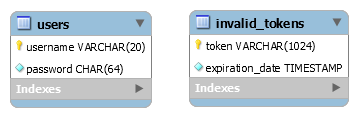
\includegraphics{AuthenticationER}
  \caption{Diagramma E/R del servizio \textit{Authentication Service}.}
\end{figure}

\section{Room Service}

\textit{Room Service} è il servizio che gestisce le \textit{chat room} di conversazione degli utenti. In particolare si occupa della creazione, eliminazione, adesione alle stanze e della persistenza dei messaggi.
Questo servizio è autonomo, non dipende da altri servizi.\\
Le risorse messe a disposizione dal servizio, specificate nella tabella \ref{tab:table_room}, permettono di:

\begin{itemize}
%
    \item \textbf{Creare} una stanza: l'utente fornisce il proprio \textit{username} e il \textit{nome} della stanza che vuole creare. Se l'operazione viene conclusa con successo il servizio risponde confermando la creazione \textit{Create} e inviando il \textit{nome} della stanza appena creata. Se l'operazione fallisce viene inviato un messaggio di errore \textit{Internal Server Error}. Se esiste già una stanza con quel nome, \textit{Room Service} risponde con messaggio di errore \textit{Conflict}.  Se \textit{username} e/o \textit{name} non sono presenti nella richiesta, il servizio restituisce il messaggio di errore \textit{Precondition Failed}.
%
    \item \textbf{Eliminare} una stanza: l'utente fornisce il proprio \textit{username} e il \textit{nome} della stanza come \textit{parametri} della richiesta. Il servizio controlla l'effettiva esistenza della stanza: se esiste il servizio conferma l'eliminazione con messaggio di accettazione \textit{OK}, altrimenti risponde con messaggio di errore \textit{Not Found}.  Se \textit{username} e/o \textit{name} non sono presenti nella richiesta, il servizio restituisce il messaggio di errore \textit{Precondition Failed}. Se l'operazione non viene conclusa correttamente il servizio risponde con \textit{Internal Server Error}.
%
    \item \textbf{Unirsi} ad una stanza: l'utente fornisce il proprio \textit{username} e il \textit{nome} della stanza come \textit{parametri} della richiesta. Se la stanza esiste, il servizio conferma la creazione della partecipazione dell'utente nella stanza \textit{Create}, altrimenti risponde con messaggio di errore \textit{Not Found}. Se \textit{username} e/o \textit{name} non sono presenti nella richiesta, il servizio restituisce il messaggio di errore \textit{Precondition Failed}. Se l'operazione non va a buon fine il servizio risponde con \textit{Internal Server Error}.
%
    \item \textbf{Abbandonare} una stanza: l'utente fornisce il proprio \textit{username} e il \textit{name} della stanza che vuole abbandonare. Se il token è valido, l'utente può disponnettersi e il servizio segna il token come non più utilizzabile, \textit{invalid}. Se i valori richiesti non sono presenti, il servizio risponde con un messaggio di errore \textit{Precondition Failed}. Se lo \textit{username} dell'utente o il \textit{name} della stanza non risultano presenti nel \textit{database}, il servizio restituisce il messaggio di errore \textit{Not Found}. Se l'operazione non viene conclusa correttamente il servizio risponde con \textit{Internal Server Error}.
%
    \item \textbf{Inviare} messaggi in una stanza: questa funzionalità permette la condivisione dei messaggi all'interno delle stanze. Infatti all'invio di un messaggio, viene creata una richiesta con \textit{username} dell'utente e \textit{content} del messaggio. Se l'operazione va a buon fine \textit{Create}, il \textit{RoomService} genera una risposta con il \textit{content} e il \textit{timestamp} del messaggio, il \textit{name} della stanza e lo \textit{username} dell'utente. Se i campi richiesti non sono presenti o non sono corretti, il servizio risponde rispettivamente con il messaggio di errore \textit{Precondition Failed}, oppure con messaggio di errore \textit{Not Found}. Se l'operazione non va a buon fine il servizio risponde con \textit{Internal Server Error}.
%
\end{itemize}

\begin{table}[H]
\centering
\resizebox{\columnwidth}{!}{%
\begin{tabular}{|l|l|c|c|c|l|}
\hline
\begin{tabular}[c]{@{}l@{}}HTTP\\ verb\end{tabular} & Resource                             & \begin{tabular}[c]{@{}c@{}}Request\\ Body\end{tabular}      & \begin{tabular}[c]{@{}c@{}}Response\\ Body\end{tabular}                      & Responses                                                    & \multicolumn{1}{c|}{Description}                                                                    \\ \hline
POST                                                & /rooms/                              & \begin{tabular}[c]{@{}c@{}}username, \\ name\end{tabular}   & name                                                                         & \begin{tabular}[c]{@{}c@{}}201, 412,\\ 500\end{tabular}      & Creazione stanza                                                                                    \\ \hline
GET                                                 & /rooms/                              & -                                                           & list of Room                                                                 & 200                                                          & Recupera la lista delle stanze                                                                      \\ \hline
DELETE                                              & /rooms/:name                         & username                                                    & name                                                                         & \begin{tabular}[c]{@{}c@{}}200, 404,\\ 412, 500\end{tabular} & Eliminazione stanza                                                                                 \\ \hline
POST                                                & /rooms/:name/participations          & username                                                    & participation                                                                & \begin{tabular}[c]{@{}c@{}}201, 404,\\ 412, 500\end{tabular} & Adesione alla stanza                                                                                \\ \hline
GET                                                 & /rooms/:name/participations          & -                                                           & list of Participations                                                       & 200                                                          & \begin{tabular}[c]{@{}l@{}}Recupera la lista delle\\ partecipazioni della stanza data\end{tabular}  \\ \hline
GET                                                 & /users/:username/participations      & -                                                           & list of Participations                                                       & 200                                                          & \begin{tabular}[c]{@{}l@{}}Recupera la lista delle\\ partecipazioni dell'utente dato\end{tabular}   \\ \hline
DELETE                                              & rooms/:name/participations/:username & -                                                           & name, username                                                               & \begin{tabular}[c]{@{}c@{}}200, 404,\\ 412, 500\end{tabular} & Abbandono della stanza                                                                              \\ \hline
POST                                                & rooms/:name/messages                 & \begin{tabular}[c]{@{}c@{}}content,\\ username\end{tabular} & \begin{tabular}[c]{@{}c@{}}content, timestamp,\\ username, name\end{tabular} & \begin{tabular}[c]{@{}c@{}}201, 404,\\ 412, 500\end{tabular} & Invio messaggio                                                                                     \\ \hline
GET                                                 & rooms/:name/messages                 & -                                                           & list of Messages                                                             & 200                                                          & \begin{tabular}[c]{@{}l@{}}Recupera la lista dei messaggi\\ presenti nella stanza data\end{tabular} \\ \hline
\end{tabular}
}
\captionof{table}{Risorse esposte dal \textit{Room Service}.} \label{tab:table_room} 
\end{table}

\begin{figure}[H]
  \centering
    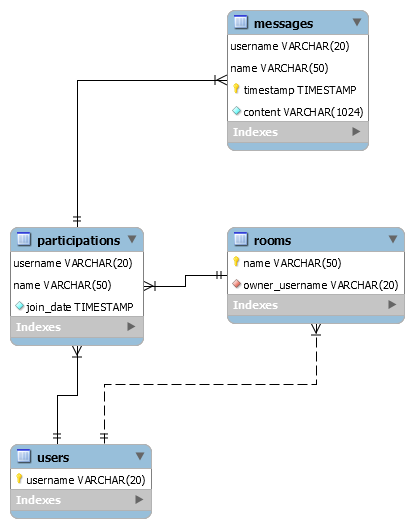
\includegraphics[scale=0.5]{RoomER}
  \caption{Diagramma E/R del servizio \textit{Room Service}.}
\end{figure}

\section{User Service}

\textit{User Service} è il servizio che gestisce il \textit{profilo} di ogni utente registrato all'applicazione. In particolare si occupa della creazione, eliminazione e aggiornamento dei profili utente.
Questo servizio è autonomo, non dipende da altri servizi.\\
Le risorse messe a disposizione dal servizio, specificate nella tabella \ref{tab:table_user}, permettono di:

\begin{itemize}
%
    \item \textbf{Creare} un utente: l'utente fornisce il proprio \textit{nome utente}, \textit{nome} e \textit{cognome}. Se l'operazione viene conclusa con successo il servizio risponde confermando la creazione con il messaggio \textit{Create} e inviando il \textit{profilo} dell'utente appena creato. Se l'operazione fallisce il servizio risponde con il messaggio di errore \textit{Internal Server Error}. Se esiste già un utente col \textit{nome utente} fornito in input il servizio risponde con il messaggio di errore \textit{Conflict}.  Se \textit{nome utente}, \textit{nome}, o \textit{cognome} non sono presenti nella richiesta il servizio risponde con il messaggio di errore \textit{Precondition Failed}.
%
    \item \textbf{Eliminare} un utente: l'utente fornisce il proprio \textit{nome utente}. Se l'operazione viene conclusa con successo il servizio risponde confermando l'eliminazione dell'utente con il messaggio \textit{(OK)} e inviando il \textit{nome utente} dell'utente appena eliminato. Se l'operazione fallisce il servizio risponde con il messaggio di errore \textit{Internal Server Error}. Se non esiste un utente con il \textit{nome utente} specificato il servizio risponde con il messaggio di errore \textit{Not Found}. Se il \textit{nome utente} non è presente nella richiesta il servizio risponde con il messaggio di errore \textit{Precondition Failed}.
%
    \item \textbf{Aggiornare} il profilo utente: l'utente fornisce il proprio \textit{nome utente} oltre al nuovo \textit{nome}, \textit{cognome} e \textit{biografia}. Se l'operazione viene conclusa con successo il servizio risponde confermando l'aggiornamento del profilo utente rispondendo con il messaggio \textit{OK} e inviando il \textit{profilo} aggiornato dell'utente che ha effettuato la richiesta. Se l'operazione fallisce il servizio risponde con il messaggio di errore \textit{Internal Server Error}. Se non esiste un utente con il \textit{nome utente} specificato il servizio risponde con il messaggio di errore \textit{Not Found}. Se \textit{nome utente}, \textit{nome}, \textit{cognome} o \textit{biografia} non sono presenti nella richiesta il servizio risponde con il messaggio di errore \textit{Precondition Failed}.
%
    \item \textbf{Recuperare} il profilo utente: l'utente fornisce il proprio \textit{nome utente}. Se l'operazione viene conclusa con successo il servizio risponde confermando l'aggiornamento del profilo utente rispondendo con il messaggio \textit{OK} e inviando il profilo dell'utente che ha effettuato  la richiesta. Se l'operazione fallisce il servizio risponde con il messaggio di errore \textit{Internal Server Error}. Se non esiste un utente con il \textit{nome utente} specificato il servizio risponde con il messaggio di errore \textit{Not Found}. Se \textit{nome utente} non \`e presente nella richiesta il servizio risponde con il messaggio di errore \textit{Precondition Failed}.
%
\end{itemize}

\begin{table}[H]
\centering
\resizebox{\columnwidth}{!}{%
\begin{tabular}{|l|l|c|c|c|c|l|}
\hline
\begin{tabular}[c]{@{}l@{}}HTTP\\ verb\end{tabular} & Resource                              & \multicolumn{1}{l|}{Header} & \begin{tabular}[c]{@{}c@{}}Request\\ Body\end{tabular}                                  & \begin{tabular}[c]{@{}c@{}}Response\\ Body\end{tabular}   & Responses                                                     & \multicolumn{1}{c|}{Description}          \\ \hline
POST                                                & /users                                & -                           & \begin{tabular}[c]{@{}c@{}}username, \\ firstName, \\ lastName\end{tabular}             & User profile                                              & \begin{tabular}[c]{@{}c@{}}201, 409, 412,\\ 500\end{tabular}  & Creazione di un utente                    \\ \hline
GET                                                 & /users/:username                      & -                           & -                                                                                       & User profile                                              & \begin{tabular}[c]{@{}c@{}}200, 404,\\ 412, 500\end{tabular}  & Recuperare il profilo di un utente        \\ \hline
PUT                                                 & /users/:username                      & -                           & \begin{tabular}[c]{@{}c@{}}firstName, \\ lastName, \\ bio, \\ visible \end{tabular}     & User profile                                              & \begin{tabular}[c]{@{}c@{}}200, 404,\\ 412, 500\end{tabular}  & Aggiornamento del profilo di un utente    \\ \hline
DELETE                                              & /users/:username                      & -                           & -                                                                                       & username                                                  & \begin{tabular}[c]{@{}c@{}}200, 404,\\ 412, 500\end{tabular}  & Eliminazione di un utente                 \\ \hline
PUT                                                 & /users/:username/access               & -                           & -                                                                                       & -                                                         & \begin{tabular}[c]{@{}c@{}}200, 500\end{tabular}  & Aggiornamento ultimo accesso              \\ \hline
\end{tabular}
}
\captionof{table}{Risorse esposte dallo \textit{User Service}.} \label{tab:table_user} 
\end{table}

\begin{figure}[H]
  \centering
    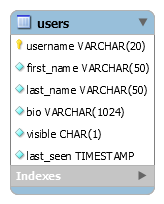
\includegraphics{UserER}
  \caption{Diagramma E/R del servizio \textit{User Service}.}
\end{figure}

\section{Web App Service}

\textit{Web App Service} è il servizio che si occupa di inoltrare le richieste effettuate dai client ai relativi servizi, di gestire la parte di aggiornamento in tempo reale dei singoli client (per es. propaganzione di un messaggio a tutti gli utenti attivi presenti all'interno di una stanza) e di servire l'applicazione web all'utente.

Per erogare tutte le funzionalit\`a esposte il \textit{Web App Service} si appoggia sui servizi di back-end descritti in precedenza. Per esempio per registrare un utente si appoggia sull'\textit{Authentication Service} per archiviare le credenziali di autenticazione e sullo \textit{User Service} per archiviare il profilo utente.

Le risorse messe a disposizione dal servizio sono specificate nella tabella \ref{tab:table_webapp}.

\begin{table}[H]
\centering
\resizebox{\columnwidth}{!}{%
\begin{tabular}{|l|l|c|c|c|c|l|}
\hline
\begin{tabular}[c]{@{}l@{}}HTTP\\ verb\end{tabular} & Resource                             & Header & \begin{tabular}[c]{@{}c@{}}Request\\ Body\end{tabular}                                & \begin{tabular}[c]{@{}c@{}}Response\\ Body\end{tabular} & Responses                                                           & \multicolumn{1}{c|}{Description}                                                                       \\ \hline
POST                                                & /register                            & -      & \begin{tabular}[c]{@{}c@{}}username, \\ firtname,\\ lastname,\\ password\end{tabular} & User                                                    & \begin{tabular}[c]{@{}c@{}}201, 412,\\ 500\end{tabular}             & Creazione utente                                                                                       \\ \hline
POST                                                & /login                               & -      & \begin{tabular}[c]{@{}c@{}}username,\\ password\end{tabular}                          & User                                                    & \begin{tabular}[c]{@{}c@{}}200, 404,\\ 412\end{tabular}             & Login utente                                                                                           \\ \hline
DELETE                                              & /logout                              & token  & username                                                                              & -                                                       & \begin{tabular}[c]{@{}c@{}}204, 401, 404,\\ 412, 500\end{tabular}   & Logout utente                                                                                          \\ \hline
GET                                                 & /rooms                               & token  & -                                                                                     & list of Rooms                                           & \begin{tabular}[c]{@{}c@{}}200, 401,\\ 404,\\ 412, 500\end{tabular} & \begin{tabular}[c]{@{}l@{}}Recupera la lista delle stanze\\ in cui l'utente non partecipa\end{tabular} \\ \hline
POST                                                & /rooms                               & token  & \begin{tabular}[c]{@{}c@{}}usernane,\\ name\end{tabular}                              & name                                                    & \begin{tabular}[c]{@{}c@{}}200, 401,\\ 404,\\ 412, 500\end{tabular} & Creazione stanza                                                                                       \\ \hline
DELETE                                              & /rooms/:name                         & token  & username                                                                              & -                                                       & \begin{tabular}[c]{@{}c@{}}204 401,\\ 404,\\ 412, 500\end{tabular}  & Eliminazione stanza                                                                                    \\ \hline
POST                                                & /rooms/:name/participations          & token  & username                                                                              & Participation                                           & \begin{tabular}[c]{@{}c@{}}201, 401,\\ 404,\\ 412, 500\end{tabular} & Adesione alla stanza                                                                                   \\ \hline
GET                                                 & /rooms/:name/participations          & token  & -                                                                                     & list of Participations                                  & \begin{tabular}[c]{@{}c@{}}200, 401,\\ 404,\\ 412, 500\end{tabular} & \begin{tabular}[c]{@{}l@{}}Recupera la lista delle\\ partecipazioni della stanza data\end{tabular}     \\ \hline
DELETE                                              & rooms/:name/participations/:username & token  & -                                                                                     & name, username                                          & \begin{tabular}[c]{@{}c@{}}200, 404,\\ 412, 500\end{tabular}        & Abbandono della stanza                                                                                 \\ \hline
POST                                                & rooms/:name/messages                 & token  & \begin{tabular}[c]{@{}c@{}}content,\\ username\end{tabular}                           & Message                                                 & \begin{tabular}[c]{@{}c@{}}201, 404,\\ 412, 500\end{tabular}        & Invio messaggio                                                                                        \\ \hline
GET                                                 & rooms/:name/messages                 & token  & -                                                                                     & list of Messages                                        & \begin{tabular}[c]{@{}c@{}}200, 401,\\ 404,\\ 412, 500\end{tabular} & \begin{tabular}[c]{@{}l@{}}Recupera la lista dei messaggi\\ presenti nella stanza data\end{tabular}    \\ \hline
GET                                                 & /users/:username                     & token  & -                                                                                     & User                                                    & \begin{tabular}[c]{@{}c@{}}200, 404,\\ 412, 500\end{tabular}        & \begin{tabular}[c]{@{}l@{}}Recupera l'utente dato\\ il suo username\end{tabular}                       \\ \hline
PUT                                                 & /users/:username                     & token  & \begin{tabular}[c]{@{}c@{}}firtname,\\ lastname,\\ bio,\\ visible\end{tabular}        & User                                                    & \begin{tabular}[c]{@{}c@{}}200, 404,\\ 412, 500\end{tabular}        & Update utente                                                                                          \\ \hline
DELETE                                              & /users/:username                     & token  & -                                                                                     & username                                                & \begin{tabular}[c]{@{}c@{}}204, 401,\\ 404,\\ 412, 500\end{tabular} & Eliminazione utente                                                                                    \\ \hline
GET                                                 & /users/:username/participations      & token  & -                                                                                     & list of Participations                                  & \begin{tabular}[c]{@{}c@{}}200, 401,\\ 404,\\ 412, 500\end{tabular} & \begin{tabular}[c]{@{}l@{}}Recupera la lista delle\\ partecipazioni di un\\ dato utente\end{tabular}   \\ \hline
\end{tabular}
}
\captionof{table}{Risorse esposte dallo \textit{User Service}.} \label{tab:table_webapp} 
\end{table}

\section{Client}
Il front-end del sistema è un'Applicazione Web realizzata in Angular e servita dal \texttt{WebAppService}.
L'applicazione si presenta con una prima pagina di \textit{login}, dove l'utente potrà inserire il suo \textit{username} e la \textit{password}. Nel caso l'utente non fosse ancora registrato, ha a possibilità di registrarsi e creare un proprio profilo.

Una volta effettuato l'accesso la pagina presenta:
\begin{enumerate*}[label=(\arabic*)]
    \item un menù laterale in cui sono visibili le stanze a cui l'utente ha ito,
    \item una funzionalità di \textit{ricerca} delle stanze,
    \item una funzionalità che permette la \textit{creazione} di nuove stanze,
    \item un bottone per il logout e la modifica del profilo utente,
    \item la chat di messaggistica che mostra i messaggi scambiati dagli utenti,
    \item un bottone che permette di vedere le informazioni riguardanti una stanza, in particolare i partecipanti alla chat e il loro profilo.
\end{enumerate*}

